\chapter{metoder}
Dette Kapitel indeholder beskrivelser af hvordan projektet er udført, og med hvilke metoder der er brugt. Yderligere indeholder kapitlet projektstyring, samt modeller der er fulgt igennem projektforløbet. 
\section{projektstyring/planlægning} 
Til projektstyring af dette projekt er der brugt en stage gate model. En stage gage model(figur \ref{fig:stage-gate}) er bestående af nogle udviklingsfaser(stages), hvor ved der er en deadline for de konkrete faser. For at komme til næste fase/stage, skal der være opfyldt nogle kriterier. Kriterierne sættes op i en tjekliste(se figur \ref{fig:stage-gate-tjekliste}), hvor de kan krydses af. Alle punkter skal være opfyldt for at komme i gennem gaten. En stage gate model er god til at få et produkt på markedet, men det har sine svagheder ved en agil udviklingsprocess. \fxnote{skriv noget omkring at i dette projekt er gatene ikke lukkede efter de er gennem gået og derved kan der gåes tilbage og rettes i projektet}
\begin{landscape}
\begin{figure}[H]
	\centering
	\includegraphics[width=1.6\textwidth]{billeder/Hovedrapport/Stage-gateP.PDF}
	\caption{Stage gate model}
	\label{fig:stage-gate}
\end{figure}
\end{landscape}
\fxnote{stage gate modellayout}

\begin{figure}[H]
	\centering
	\includegraphics[width=0.7\textwidth]{billeder/Hovedrapport/Stagegatetjekliste.PDF}
	\caption{Stage gate model}
	\label{fig:stage-gate-tjekliste}
\end{figure}

%\begin{sidewaysfigure}
%\begin{figure}[H]
%	\centering
%	\includegraphics[width=0.6\textwidth]{billeder/Hovedrapport/Stage-gateP.PDF}
%	\caption{Stage gate model}
%	\label{fig:moscow}
%\end{figure}
%\end{sidewaysfigure}



%\begin{figure}
%  \begin{sideways}
%    \begin{minipage}{27.5cm}
%      \includegraphics[width=0.6\textwidth]{billeder/Hovedrapport/Stage-gateP.PDF}
%    \end{minipage}
%  \end{sideways}
%  \centering
%  \caption[Caption]{Caption.}
%  \label{pic:picture}
%\end{figure}
\subsection{Agil udviklingsprocess}
I en agil arbejdsprocess er der konstant fokus på at målrette og prioritere arbejdet mod det, der giver mest værdi for projektet og kunden. Det vil sige at der løbende prioriteres mellem opgaverne, hvorefter det er vigtigt at der hele tiden planlægges og revurderes delopgaverne. Det gør at projektets produkt, resultater evalueres og testes løbende, hvilket danner grundlag for prioriteringen af opgaverne der skal løses i den næste periode. Til at sikre at arbejdsressourcerne der har været tilrådighed er blevet brugt på den mest effektive måde, er der brugt elementer fra SCRUM. SCRUM er en iterativ arbejdsmetode, hvor  der er iterationer(sprints) som i dette projekt har haft en periode på en uge. Til at holde styr på arbejdsressourcerne til opgaverne, er der i projektet brugt \textit{Pivotaltracker}. 
I Pivotaltracker defineres projektets arbejdsopgaver, hvorefter de tildeles point alt efter hvor stor arbejdsbyrden er. De enkelte opgaver prioriteres herefter i projektets backlog, hvor Pivotaltracker automatisk tilføjer opgaver til den igangværende sprint udfra den nuværende “velocity”. En ny sprint påbegyndes automatisk når en ny uge starter.

Det betyder, at der er fuldstændig styr på om projektet går for langsomt, eller om udviklingen af projektet er godt med. Dette kan holdes op i mod den tidligere nævnte stage gate model.

Herudover giver Pivotaltracker mulighed for en komplet log over projektets udførte opgaver og afsluttede sprints. Her kan man se hvilke opgaver der er udført i hvilken uge. I projektet anvendes dette som logbog over udførte arbejdsopgaver.

En opgave kan have forskellige states, som definerer dens status. Når en opgave er afsluttet kan den afleveres til review, hvor den herefter enten kan godkendes eller afvises. Dette er særligt anvendeligt i projektets udviklingsfase, hvor en feature kan testes og godkendes af et andet projektmedlem. Figur \ref{fig:pt_sprints}  viser et overblik over tidligere sprints, hvor figur \ref{fig:pt_currentsprint} viser en igangværende sprint med opgaver der er godkendt, afsluttet og ikke færdiggjorte endnu.

\begin{figure}[htbp] \centering
\begin{minipage}[b]{0.48\textwidth} \centering
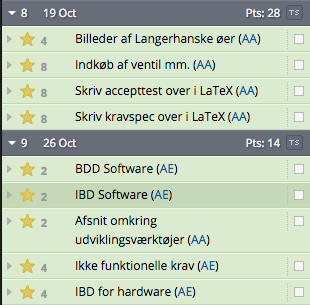
\includegraphics[width=1.00\textwidth]{billeder/pt_previous_sprints} % Left picture
\end{minipage} \hfill
\begin{minipage}[b]{0.48\textwidth} \centering
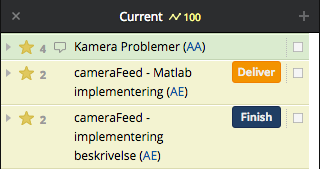
\includegraphics[width=1.00\textwidth]{billeder/pt_current_sprint} % Right picture
\end{minipage} \\ % Captions og labels
\begin{minipage}[t]{0.48\textwidth}
\caption{Færdiggjorte sprints} % Left caption and label
\label{fig:pt_sprints}
\end{minipage} \hfill
\begin{minipage}[t]{0.48\textwidth}
\caption{Igangværende sprint} % Right caption and label
\label{fig:pt_currentsprint}
\end{minipage}
\end{figure}
\fxnote{overvej om vi skal have andre billeder med en højere vilocity}

\section{De fire udviklingsfaser}
Under udviklingen af projektet, er der gennem gået fire faser. Den første fase i projektet har været koncept analyse. Koncept analysen bestod af litteratursøgning omkring langerhanske øer, dette blev gjort for at opnå tilstrækkelig viden omkring størrelserne, deres egenskaber mm. Der blev også søgt allerede eksisterende sorteringsmetoder, som blev anvendt på det daværende tidspunkt. Dette var primært for at opnå erfaring inden for området på kort tid. Efter litteratursøgningen blev et overordnet koncept etableret i samarbejde med kunden(\textit{Søren Gregersen}). samtidigt med Koncept analysen, blev det parallelt med tænkt på produktionen af produktet. Grunden til dette er, at det vil være uanvendeligt at opnå løsninger, som er for besværlige at producerer. 

Den anden fase består af kravspecifikationen, hvilket er udarbejdet i tæt samarbejde med kunden. En kravspecifikation sikre at kunde og projekt udviklere er enige om projektets udformning. I kravspecifikationen er der brugt usecasediagram, samt fully dresseds til hver usecase. Der laves fully dresseds, for at klaregøre normal forløbet til hver usecase, samt undtagelser og undvigelser til dem. Derudover det også i kravspecifikationen at der er specificeret ikke funktionelle krav og kvalitetskrav. Samtidigt med kravspecifikationen er der udarbejdet en accepttest. Denne test sikres at alle krav, der er bestemt i samarbejde med kunde er opnået. I acceptesten er det beskrevet hvordan hver enkelt krav skal testes, hvilket udføres før produktet afleveres til kunden se afsnit \ref{subsec:krav} for eksempler.

Den tredje fase i projektet har været Design, hvor der udfra kravspecifikationen er lavet over ordnet diagrammer. Diagrammerne bruges til at beskrive systemet over ordnet, men også i små delsystemer. Det er diagrammerne der bruges til at udvikle videre fra. Desuden er de Enkelte komponenters specifikationer beskrevet i designet. Derfor er det i denne fase der er bestilt komponenter til projektet, se afsnit \ref{subsec:design} for eksempler. 

I den fjedre fase er der blevet produceret en prototype. Derfor er der i denne fase kodet, monteret og testet. Hvilket er sket på iterativ metoden, så der først kodes, monteres og derefter testes det. Dette er gjort ved så små delelementer som muligt, for at være sikker på at hver delelement virker inden det sættes sammen. Se afsnit \ref{subsec:Implement} for eksempler af denne fase. 

De fire udviklings faser brugt i projektet kan illustreres som på figur \ref{fig:v-model}, har haft sine fordele og ulemper. Fordelene er at der sikres dokumentation af projektet fra starten, samt at der hele tiden tænkes på slutresultatet og slutbrugeren. Ulemperne er at der er meget dokumentation, der bliver ændret fra hvad det var i starten af projektet. På den måde kan man godt tro at det er spild af tid, men det sikre samtidigt at projektet bliver vel dokumenteret og gennemtænkt fra starten.

\begin{figure}[H]
	\centering
	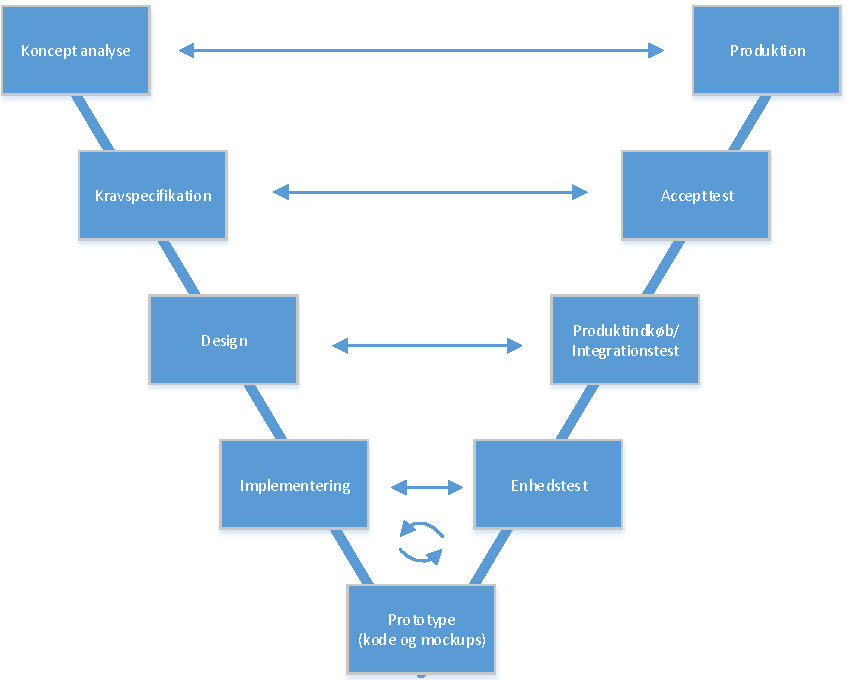
\includegraphics[width=0.7\textwidth]{billeder/Hovedrapport/V-model.PDF}
	\caption{Stage gate model}
	\label{fig:v-model}
\end{figure}

I modsætning til v-modelle findes der også vandfaldsmodellen, hvor hver enkelt fase bliver lavet færdig før der gås videre til den næste. Dette medfører ofte nedprioritering af test og andre sene deadlines i projektet, grundet at tidligere tidsplaner er skreden.

\subsection{Koncept analyse}
hmm...
 
\subsection{Kravspecifikation og accepttest}
\label{subsec:krav}
For at vise at der er brugt de beskrevne metoder ovenfor, er der valgt at tage eksempler med i rapport. %for at eftervise de fire udviklingsfaser projektet har været i gennem.

\subsubsection{Aktør beskrivelse}
Systemets primære aktør er operatøren, som står for påfyldning af celler, start og stop af sorteringsprocessen. Operatøren har mulighed for at interagere med systemet via en grafisk brugergrænseflade. Systemets sekundære aktør er kameraet og PC’ens filsystem. Kameraet er systemets interface til detektion af de Langerhanske øer. Filsystemet er hvor der løbende gemmes en log over sorteringsprocessen.

\subsection{Use Case Diagram}
I Use Case diagrammet (figur: \ref{fig:usecase}) er der vist, hvilke use cases systemet \textit{The Cell Collector} består af. Yderligere er det vist, hvilke aktører der initiere de enkelte use cases. På venstre side er systemets primære aktør \textit{operatøren} vist, mens systemets sekundære aktører \textit{kamera} og \textit{database} er placeret i højre side. 

\begin{figure}[H]
	\centering
	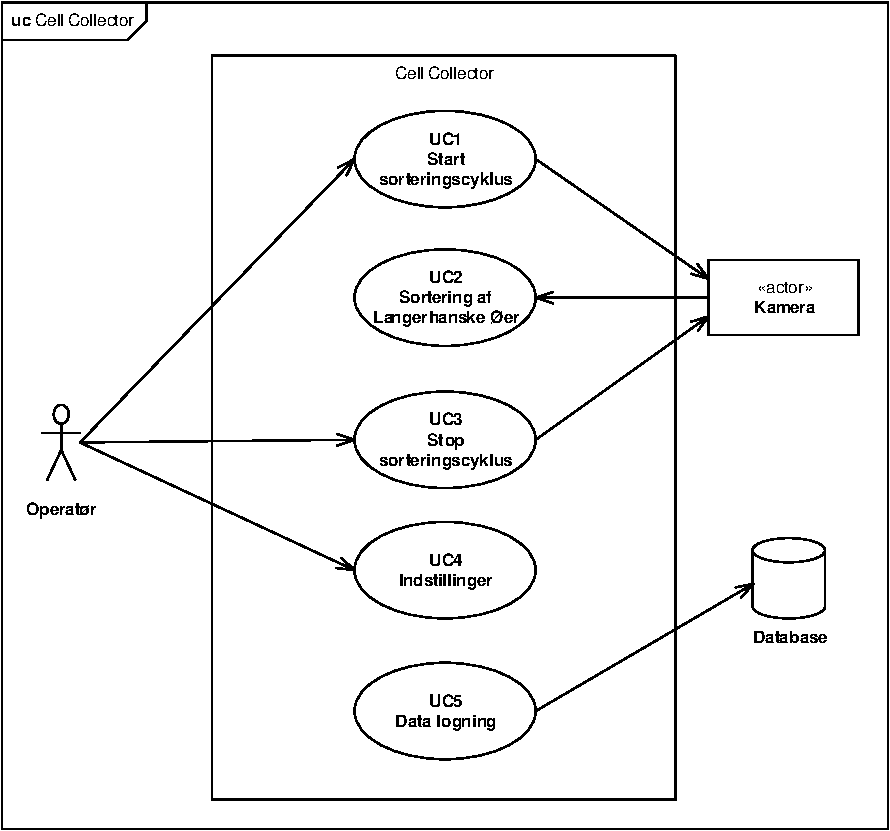
\includegraphics[width=1\textwidth]{billeder/UC_CellCollector.pdf}
	\caption{Use Case diagram for The Cell Collector}
	\label{fig:usecase}
\end{figure}
Efter use case diagrammet var færdigt, blev der udarbejdet fully dressed use cases som kan ses på nedenstående tabel. Tabellen beskriver normalforløbet og undtagelser for \textit{Start sorteringscyklus}, som er den første use case på diagrammet. 
\newpage 

\label{uc:1}
\begin{center}
		\begin{longtable}{ | m{4cm} | m{8cm}| } 
			\hline
			Mål & Start sorteringscyklus \\ 
			\hline
			Initiering &  Use casen initieres af operatøren\\
			\hline
			Aktør & 
			Primær: Operatør
			
			 Sekundær: Kamera			  \\ 
			\hline
			Startbetingelser & The Cell Collector programmet er startet på computeren \\ 
			\hline	
			Slutbetingelser ved succes & Systemet starter med sorteringen af Langerhanske øer \\
			\hline
			Slutbetingelser ved undtagelse & N/A \\
			\hline
			Normalforløb & \begin{enumerate}
				%\setlength\itemsep{0cm} % Decrease line distance
				\item Operatør fylder celleopløsningsbeholderen
				\item Celleopløsningsbeholderen er fyldt
				\item Operatør starter sorteringscyklus ved at klikke på [Start]
				\subitem [Undtagelse 1: Wastebeholder er fyldt] 
				\item Systemet initialiserer Arduinoen
				\subitem [Undtagelse 2: Ingen forbindelse til Arduino]
				\item Systemet kontrollerer celleopløsningsbeholderen ved at konvertere spændingen (\SI{}{\volt})  til \SI{}{\milli\litre}, og vise beholderens indhold (\SI{}{\milli\litre}) på GUI
				\item Systemet initialiserer kameraet
				\subitem [Undtagelse 3: Kameraet initialiserer ikke]
				\item Systemet tænder for kamera lyset
				\item Systemet tænder for pumpen
				
			\end{enumerate} \\ 
			\hline
			Undtagelser & [Undtagelse 1: Wastebeholder er fyldt] 
			
			\begin{enumerate}
			\item Systembesked: Tøm venligst Wastebeholder før start
			\item Operatøren trykker “OK”
			\item Systemet fortsætter opstartprocessen
			\end{enumerate} 
			
			[Undtagelse 2: Ingen forbindelse til Arduino]
			
			\begin{enumerate}
			\item 1.	Systembesked: Ingen forbindelse til Arduino, kontrollér forbindelser.
			\end{enumerate} 
	
			[Undtagelse 3: Kameraet initialiseres ikke]
			
			\begin{enumerate}
			\item System fejlmeddelse: Kameraet er ikke initialiseret:
			\item Genstart initialisering af Kameraet
			\end{enumerate} \\
			\hline
		\end{longtable}
	\end{center}

Efter at normalforløbet og undtagelserne er defineret, blev acceptesten lavet for den givne use case. Til hvert punkt i normalforløbet er der forberedt en test, som indeholder et krav nr, handling dvs det der skal gøres for at starte testen. Derudover er der forventet resultat, som skal ske for at testen kan godkendes, testmetode beskriver hvordan testen skal udføres og hvordan den godkendes.

\begin{center}
		\begin{longtable}{ | m{4cm}| m{8.5cm}|} 
			\hline
			\textbf{Krav nr.} & 1.1 \& 1.2    \\ 
			\hline
			\textbf{Handling} &  Operatør fylder celle-opløsnings-beholderen   \\
			\hline
			\textbf{Forventet resultat} &  Celle opløsningsbeholderen er fyldt  \\
			\hline
			\textbf{Testmetode}  &  Celle opløsningsbeholderen fyldes med væske  \\
			\hline
			\textbf{Resultat}  &    \\
			\hline
			\textbf{Angiv godkendelse} &     \\
			\hline
			\textbf{Initialer} &     \\
			\hline
			\textbf{Dato} &    \\
			\hline
		\end{longtable}
	\end{center}
	
	
	\begin{center}
		\begin{longtable}{ | m{4cm}| m{8.5cm}|} 
			\hline
			\textbf{Krav nr.} & 1.3    \\ 
			\hline
			\textbf{Handling} &  Operatør starter sorteringscyklus ved at klikke på [Start]  \\
			\hline
			\textbf{Forventet resultat} &  Opstarts processen i gang sættes.  \\
			\hline
			\textbf{Testmetode}  & Knappen [Start] trykkes, observeres ved tekstboks på GUI, med teksten \textit{systemet starter op}.   \\
			\hline
			\textbf{Resultat}  &    \\
			\hline
			\textbf{Angiv godkendelse} &     \\
			\hline
			\textbf{Initialer} &     \\
			\hline
			\textbf{Dato} &    \\
			\hline
		\end{longtable}
	\end{center}
	
	\begin{center}
		\begin{longtable}{ | m{4cm}| m{8.5cm}|} 
			\hline
			\textbf{Krav nr.} & 1.4    \\ 
			\hline
			\textbf{Handling} &  Systemet initialisere Arduinoen   \\
			\hline
			\textbf{Forventet resultat} &  Arduino initialiseret signal modtages og gives til GUI  \\
			\hline
			\textbf{Testmetode}  & Det observeres på GUI at Arduinoen er initialiseret, i en tekstboks med testen \textit{Arduino er initialiseret}.   \\
			\hline
			\textbf{Resultat}  &    \\
			\hline
			\textbf{Angiv godkendelse} &     \\
			\hline
			\textbf{Initialer} &     \\
			\hline
			\textbf{Dato} &    \\
			\hline
		\end{longtable}
	\end{center}
	
	\begin{center}
		\begin{longtable}{ | m{4cm}| m{8.5cm}|} 
			\hline
			\textbf{Krav nr.} & 1.5    \\ 
			\hline
			\textbf{Handling} &  Systemet kontrollerer celle-opløsnings-beholderen  \\
			\hline
			\textbf{Forventet resultat} &  Antal ml i celleopløsningsbeholderen vises på GUI.  \\
			\hline
			\textbf{Testmetode}  & Der hældes 100 ml i celleopløsningsbeholderen, det observeres på GUI om der vises 100 ml $\pm$ 10 ml   \\
			\hline			
			\textbf{Resultat}  &    \\
			\hline
			\textbf{Angiv godkendelse} &     \\
			\hline
			\textbf{Initialer} &     \\
			\hline
			\textbf{Dato} &    \\
			\hline
		\end{longtable}
	\end{center}	
	
Resten af acceptesten for use case 1 kan ses i projektdokumentationen \fxnote{hvordan skal der refereres her til ?} 

\subsection{Design}
\label{subsec:design}
I dette afsnit er der givet et eksempel på hvordan projektet er gået fra krav til en måde at løse projektet på. Der er blandt andet brugt BDD, IBD, flowchart samt sekvendsidagrammer til at beskrive funktioner og sammenhænge i projektet. 

\subsubsection{BDD og IBD for hardware}
Nedenstående BDD \ref{fig:bdd_Hardware} giver et over ordnet overblik i, hvad \textit{The cell collector} indeholder af hardware elementer. Hierarkiet starter øverst med \textit{The cell collector}, som indeholder tre mindre hardware dele. styreenheden der er defineret som en arduino, den indeholder de elementer arduinoen styrer bla motor shieldet. Motor shieldet indeholder yderligere to dele, som den styrer. Det vil sige at pumpen og ventilen bliver styret i gennem motor shieldet. Udover styreenheden er der også ikke elektriske dele, som beholdere og førringsveje til opløsningen med langerhanske øer. Til sidst er kameraet også en af de 3 under dele til \textit{The cell collector}.

\begin{figure}[H]
	\centering
	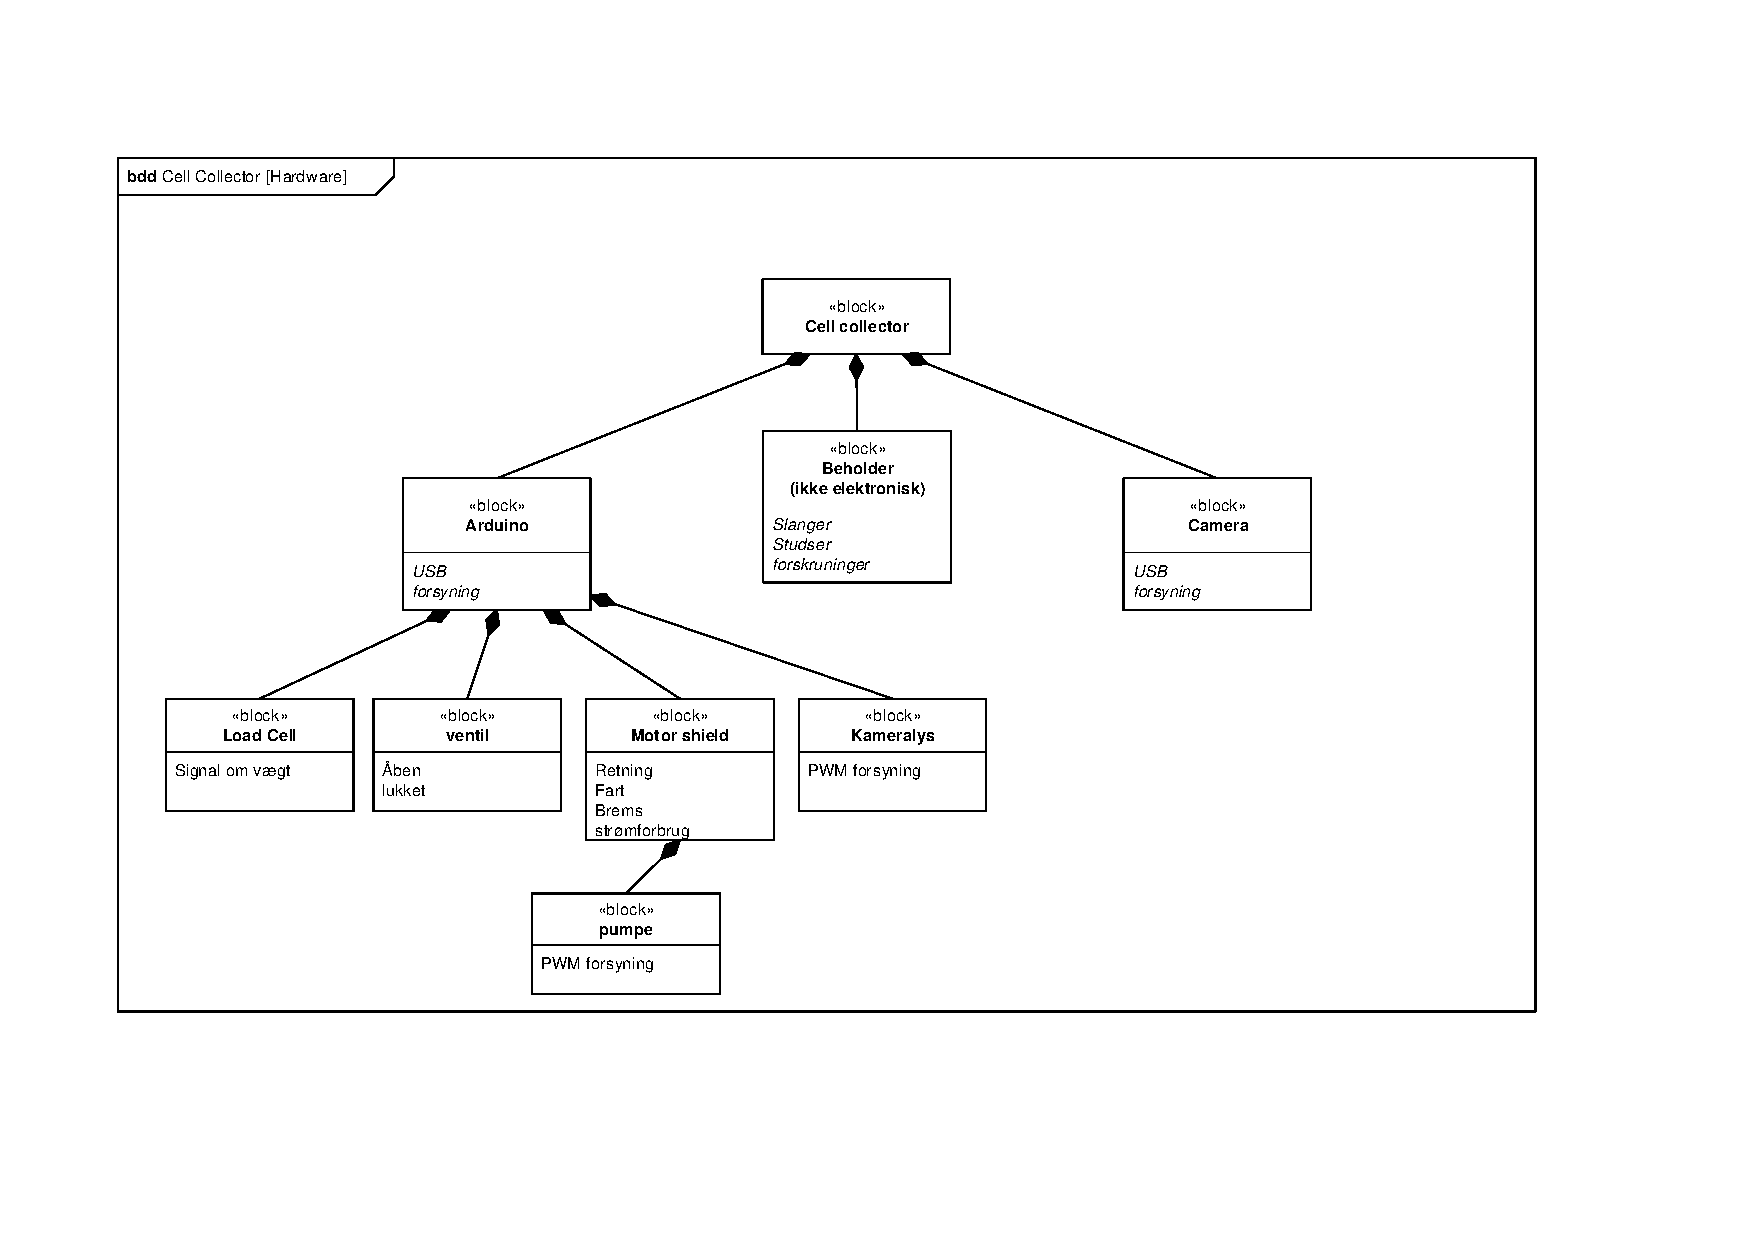
\includegraphics[width=1\textwidth]{pdf/BDD_Hardware.pdf}
	\caption{BDD - Cell Collector [Hardware]}
	\label{fig:bdd_Hardware}
\end{figure}

Nedenstående IBD \ref{fig:ibd_Hardware} beskriver mere præcist, hvordan de forskellige komponenter interagerer med hinanden på. Diagrammet er brugt til, at der tidligt i udviklingsforløbet bliver defineret hvilke spændinger og signaltyper systemet skal indeholde. Systemet skal indeholde bestemte typer for, at kunne kommunikere med de interne dele.


\begin{figure}[H]
	\centering
	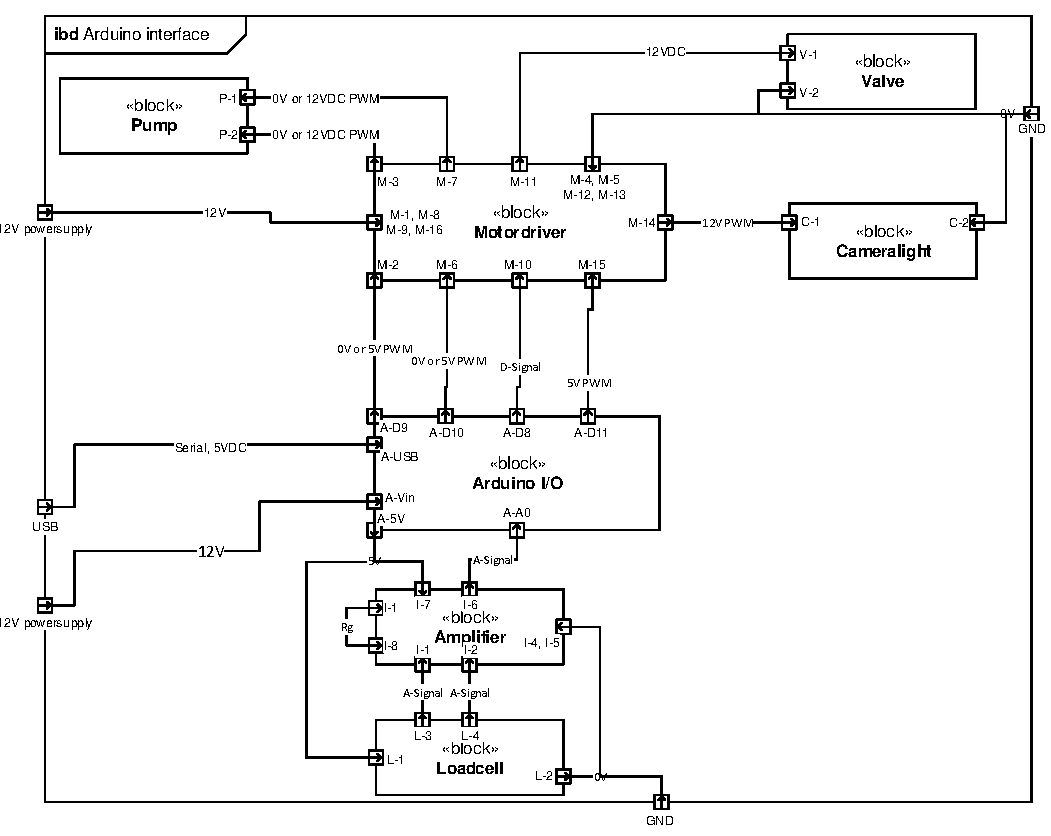
\includegraphics[width=1\textwidth]{pdf/IBD_Hardware(Arduino).pdf}
	\caption{IBD - Cell Collector [Hardware]}
	\label{fig:ibd_Hardware}
\end{figure}

Til ovenstående diagrammer kan der findes tabeller til at beskrive signalerne og blokbeskrivelser. \fxnote{reference til projektdokumentation}

Ydermere kan der ses specifikationerne for vægtcellen er stillet op og hvilke overvejelser der er gjort ved dette komponent.
\subsubsection{Vægtcelle}
\label{subsec:loadcell}
Vægtcellen skal bruges til at kontrollere om, der er væske i celleopløsningsbeholderen.

\textbf{Specifikationer for Vægtcelle[\citet{DH7}]:} 
\begin{center}
		\begin{longtable}{ | m{6.5cm} | m{6.5cm}| } 
			\hline
			\textbf{Specifikation} &\textbf{Værdi} \\ 
			\hline
			\textbf{Max belastning:} & 1 kg \\ 
			\hline
			\textbf{Anbefalet arbejdsspænding} & 3-12V \\ 
			\hline
			\textbf{Output} & 1.0mV/V$\pm$0.15mV/V \\ 
			\hline
		\end{longtable}
\end{center}

Den indkøbte vægtcellen kan veje op til 1 kg, hvilket dækker vægten for celleopløsningsbeholderen på 250ml + beholderens vægt.

Til sidst i design dokumentet er der lavet sekvensdiagrammer for, at få overblik over de sekventielle dele af systemet til hver use case se figur \ref{fig:sekvendisgr} for et eksempel.
\begin{figure}[H]
	\centering
	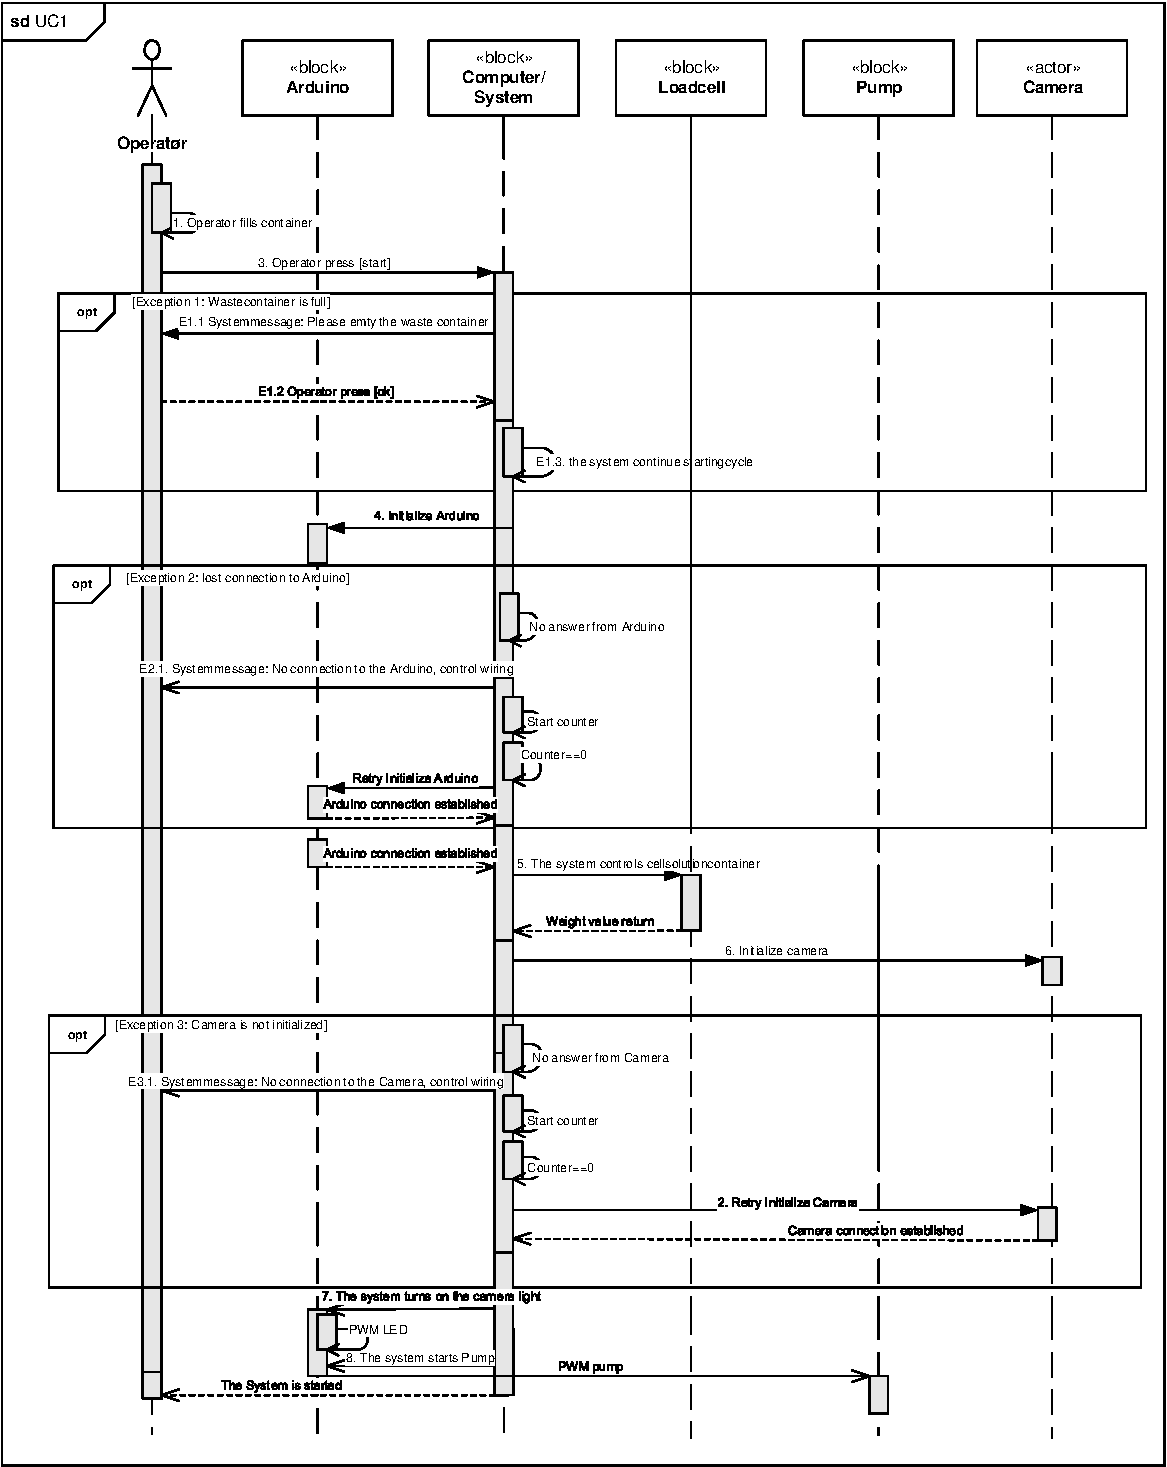
\includegraphics[width=1\textwidth]{pdf/UC1_cropped.pdf}
	\caption{Sekvensdiagram for usecase 1}
	\label{fig:sekvendisgr}
\end{figure}


\subsection{Implementering og enhedstest}
\label{subsec:Implement}
I dette afsnit er der vist et eksempel på hvordan delene er implementeret ved at vise vægtcellen for både hardware og software.

\subsubsection{Hardware}
afventer samuel
\subsubsection{Software}
afventer samuel


-samarbejdsaftaler

handlingsplan kontra tidsplan fra forprojektet

lavet efter design dokumentet er færdig bla bla bla. konrekte opgaver er lavet

- indsæt eksempel med loadcelle
